\section{Oracle Cloud Cluster Deployment Experiment}
\label{sec:mumbai-experiment}

We deployed the connection-replacement mechanism in an Oracle Cloud cluster
running Kubernetes in a development environment and first exercised it with 20,000
registered subscriptions. This initial experiment
measures live probe promotion, subscription reassociation, handoff timing, and
post-migration topology. The controlled scale-out and policy comparisons in
Section~\ref{sec:locked-evidence} use a simulator and are reported separately.
Sections~\ref{sec:mumbai-startup} and~\ref{sec:live-dql-scaleout} report
separate isolated trials, including selective DQL migration during delivery
and a one-to-four-Pod scale-out sequence.

\subsection{Deployment and Execution}

The deployment contained ten subscriber-service pods. Ten client processes
each maintained five active persistent connections, with 400 subscriptions per
connection, and one additional subscription-free probe. The inventory had
four event-type groups, each with 5,000 subscriptions. Every client loaded the
same frozen DQL checkpoint, with exploration disabled and no training updates
during evaluation. The deployed action profile admitted rebalancing and
migration but masked connection scale-up and scale-down.

Each client could execute at most one guarded connection migration. A selected
probe was promoted only after telemetry and execution checks passed. The
executor then reassociated the source connection's 400 subscriptions, drained
in-flight delivery, retired the source socket, and opened a fresh
subscription-free probe. Subscription receipts and server-reported counts
were checked against the client assignment. After execution, each process
held its topology for 1,800 seconds and checked it again before shutdown.
The statistical unit is one deployment run, containing ten client migrations.

\begin{table}[t]
  \caption{Measured Oracle Cloud cluster deployment results. Handoff and drain statistics
  summarize ten executed connection migrations. Drain wait is part of handoff
  time, not an additional independent interval.}
  \Description{Live experiment with ten pods, twenty thousand subscriptions,
  ten successful connection replacements, four thousand moved subscriptions,
  and exact final topology in all ten clients. Handoff median is 14.498 seconds;
  drain-wait median is 7.347 seconds.}
  \label{tab:mumbai-live-results}
  \centering
  \small
  \begin{tabular}{p{0.60\linewidth}r}
    \toprule
    Measurement & Observed value \\
    \midrule
    Subscriber-service pods / client processes & 10 / 10 \\
    Registered and attached subscriptions & 20,000 \\
    Active persistent connections / probes & 50 / 10 \\
    Executed full-connection migrations & 10 \\
    Subscriptions moved per migration / total & 400 / 4,000 \\
    Handoff time: minimum / median / maximum (s) & 7.898 / 14.498 / 101.563 \\
    Drain wait: minimum / median / maximum (s) & 1.264 / 7.347 / 92.450 \\
    Exact final topologies after 1,800 s & 10/10 \\
    Recorded deliveries / processed and acknowledged & 114,986 / 113,149 \\
    Processing failures / ACK failures / NACK failures & 0 / 0 / 0 \\
    Recorded duplicate candidates & 0 \\
    Independent pod samples / collection errors & 310 / 0 \\
    Pod restart increase during observation & 0 \\
    \bottomrule
  \end{tabular}
\end{table}

\subsection{Observed Handoff and Topology}

Table~\ref{tab:mumbai-live-results} shows that all ten clients replaced one
active connection and moved its full subscription set. In every case, the
destination was the retained probe, the other four active connections remained
in place, and the replacement probe had no subscriptions. The final checks
confirmed all 2,000 subscriptions and five active connections in each client
after the 30-minute hold. Thus, 4,000 subscriptions changed their transport
association while the complete 20,000-subscription client population remained
accounted for.

Handoff duration ranged from 7.898 to 101.563 seconds, with a median of
14.498 seconds. The corresponding source-drain waits ranged from 1.264 to
92.450 seconds, with a median of 7.347 seconds. The range is important:
replacement time includes waiting for outstanding work, not just opening
a socket. This run deliberately used eight processing workers
and a two-second processing delay per event in each client. Those settings
exercise handoff under a bounded client drain rate. The endpoint is handoff
behavior under this processing limit, rather than maximum Pod throughput.

\begin{figure}[!htbp]
  \centering
  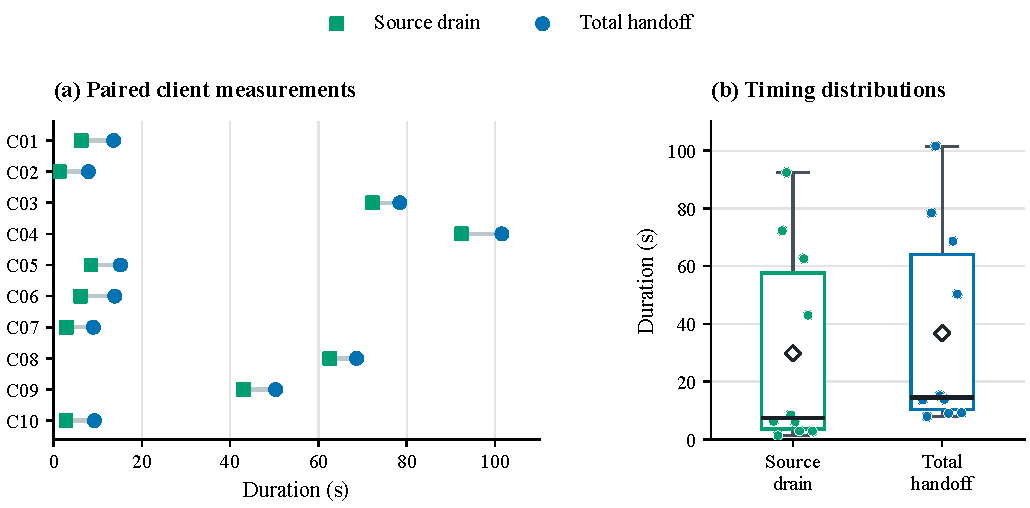
\includegraphics[width=\textwidth]{figures/mumbai-handoff-boxplots.pdf}
  \caption{Measured Oracle Cloud cluster migration timing. Left: paired source-drain and
  total-handoff durations for each of the ten client migrations. Right:
  quartile boxes with median lines, mean diamonds, and all ten observations;
  whiskers extend to observations within 1.5 interquartile ranges. These are
  ten migrations in one cluster run, not ten independent cluster trials.}
  \Description{Paired duration markers and box plots show source drain and
  total handoff for ten clients. Longer handoffs coincide with longer source
  drain waits. Drain is a component of
  total handoff, not an additional duration.}
  \label{fig:mumbai-handoff-distributions}
\end{figure}
\FloatBarrier

Figure~\ref{fig:mumbai-handoff-distributions} retains the pairing that a
summary median cannot show. For client $u$, the interval between its two
markers is $T^{\mathrm{handoff}}_u-T^{\mathrm{drain}}_u$, the measured non-drain remainder of
the handoff; it is not an estimate of network latency alone. The box extends
from the sample's first to third quartile, so the interquartile range describes
the central half of the timings. All points, including the long-duration
observations, remain visible. Longer handoffs coincide with longer source
drains, consistent with the receipt-gated mechanism waiting for outstanding
work. These are within-run timing distributions; their scope is the observed
deployment, without a between-deployment confidence interval.

An independent collector retained 31 observations of each of the ten pods
over approximately 2,422 seconds. All pods remained Ready, with unchanged
pod, image, and process identities and no restart increase. These observations
establish operational continuity over this observation period. Long-term
availability is outside the measurement window.

\subsection{Event Accounting and Interpretation}

The clients recorded 114,986 deliveries and 113,149 processed and acknowledged
events, with no recorded processing, acknowledgement, or negative-
acknowledgement failures. The final difference is 1,837 deliveries whose
eventual status is not resolved by these counters. Zero duplicate candidates
describes the configured observation window, rather than an exactly-once
delivery guarantee. The run consumed existing queued work without a matched
static-policy workload. Its contribution is measured probe-based connection
replacement with 20,000 subscriptions: subscription reassociation, source
retirement, and the connection layout after the hold period. Its endpoints
are handoff execution and topology retention, not a comparative backlog-drain
rate.

The private evidence archive retains the frozen-policy and inventory hashes,
per-client decision and topology records, delivery counters, and independent
pod observations. A recursive manifest covers 134 files; aggregate values in
Table~\ref{tab:mumbai-live-results} come from the active-execution gate and
pod-observation summaries, not from simulator output.

\subsection{Concentrated Placement and Startup Under Load}
\label{sec:mumbai-startup}

We conducted a separate Oracle Cloud cluster experiment with an isolated subscriber
Deployment and Service to examine what happens when persistent TCP connections remain on one Pod. In an initial 4,000-subscription static calibration, ten delivery
connections and two probes terminated on one Pod. Adding three Ready Pods did
not relocate these sockets: the source retained all twelve established
connections, while each added Pod had none. The clients nevertheless received
and acknowledged events while subscription activation was still progressing.
Full activation took approximately 1,398.4 seconds; the completed run reconciled
137,008 observed deliveries with confirmed ACKs. This shows the difference between having server capacity and reaching it
through existing persistent connections.

A later frozen-DQL test used 2,000 other subscriptions, divided
equally among four event-type groups. One client attached five connections,
each carrying 400 subscriptions, to the single source Pod. Three destination
Pods became Ready before standby bindings were activated. The client used
32 processing workers without an artificial processing delay, ten message
permits per subscription, and a window of 32 outstanding activation requests.
Exact lifecycle records used batched SQLite transactions with FULL
synchronization and a mandatory flush at measurement and closure boundaries.
The earlier calibration used a different subscription population and recorder
settings. The two timing records are therefore reported as separate
experiments rather than a matched static-policy comparison.

\begin{table}[!htbp]
  \caption{Measured isolated Oracle Cloud cluster connection-rebalancing qualification.
  These values describe one live run, distinct from the earlier
  20,000-subscription deployment.}
  \Description{Four available Pods, two thousand subscriptions, five active
  connections, three migrations of four hundred subscriptions, and exact
  reconciliation of seventy-three thousand six hundred thirty-nine observed
  deliveries. The source population falls from two thousand to eight hundred.}
  \label{tab:mumbai-isolated-recovery}
  \centering
  \small
  \begin{tabular}{p{0.65\linewidth}r}
    \toprule
    Measurement & Observed value \\
    \midrule
    Available Pods / subscribed Pods before and after & 4 / 1 and 3 \\
    Subscriptions / active connections / probe & 2,000 / 5 / 1 \\
    Time to 50\% / 90\% / full activation (s) & 238.066 / 388.139 / 426.305 \\
    Committed connection migrations / subscriptions moved & 3 / 1,200 \\
    Source subscriptions before / after & 2,000 / 800 \\
    Final subscribed-Pod populations & 800, 800, 400 \\
    Handoff times, in execution order (s) & 10.878, 10.992, 10.648 \\
    Source-drain waits, in execution order (s) & 6.069, 6.174, 6.848 \\
    Delivered / processed / receipt-confirmed ACKs & 73,639 / 73,639 / 73,639 \\
    Unresolved observed attempts at closure & 0 \\
    Recorded ACK failures / duplicate candidates & 0 / 0 \\
    \bottomrule
  \end{tabular}
\end{table}

The frozen controller committed three complete connection replacements,
each moving 400 subscriptions through a retained probe. The source population
fell from 2,000 to 800, a reduction of
$(2{,}000-800)/2{,}000=60\%$. Two destination Pods acquired 400 and 800
subscriptions. The active-connection count remained five, and all 2,000
subscriptions were confirmed in the final topology after the two-minute hold.
The migrations therefore changed which Pods served these subscriptions
without increasing the client's active-connection count.

\begin{figure}[!htbp]
  \centering
  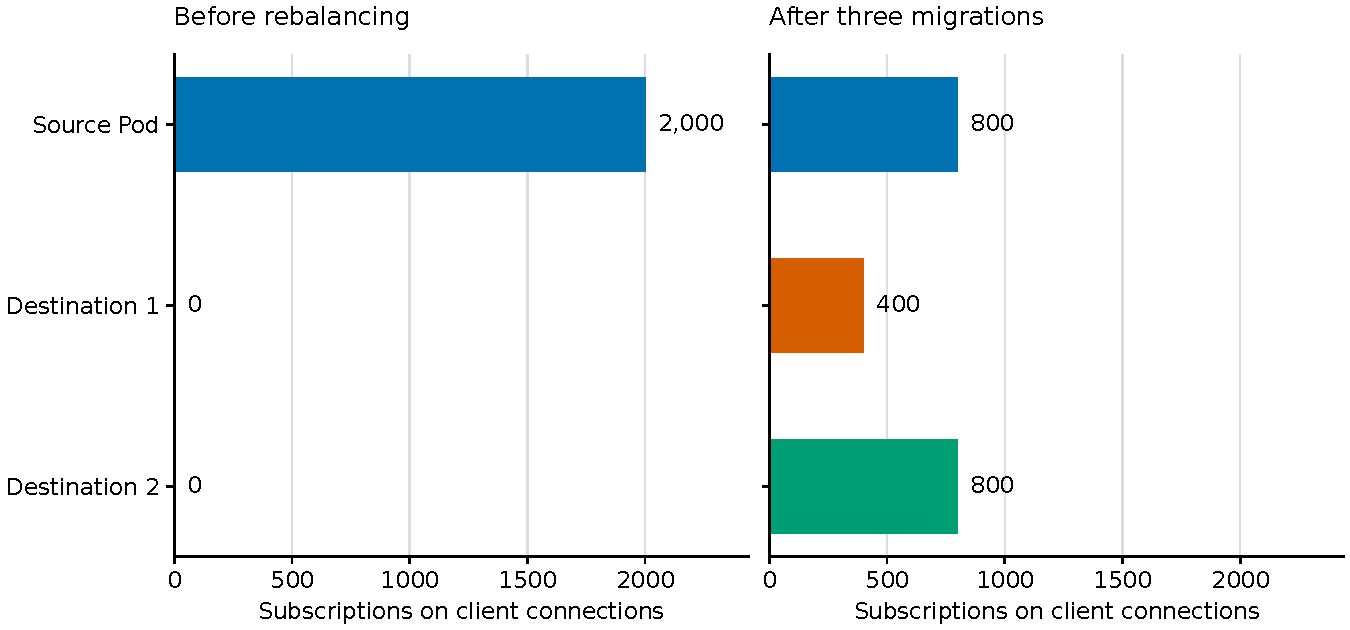
\includegraphics[width=\textwidth]{figures/observed-pod-redistribution.pdf}
  \caption{Verified client subscription placement before and after three
  frozen-DQL connection migrations in the Oracle Cloud cluster. Bars aggregate the client's
  receipt-confirmed bindings by serving Pod. Initial zeros mean no bindings
  belonging to this client, not a measurement of every cluster subscription.
  Both panels account for the same 2,000 subscriptions and five connections.}
  \Description{The initial source has two thousand subscriptions. After
  rebalancing it has eight hundred; two destinations have four hundred and
  eight hundred. No subscription is removed from the population.}
  \label{fig:mumbai-isolated-placement}
\end{figure}
\FloatBarrier

Figure~\ref{fig:mumbai-isolated-placement} shows the main operational effect:
newly available capacity becomes reachable by moving subscription-bearing
connections. It reports verified connection endpoints, rather than estimating changes
between observations. A probe was first resampled because it did not
offer an admissible improvement. Eleven later decision intervals selected
stay while backlog telemetry was incomplete; migration resumed when the
observation checks passed. The online and target network parameters remained
identical to the loaded checkpoint, while valid transitions were retained.

\subsubsection{Activation and Delivery Coexistence}

For subscription $k$, let $t_k^{\mathrm{send}}$ be activation submission time and $t_k^{\mathrm{ready}}$ its
successful receipt time, relative to the start of activation. At elapsed
time $s$ in seconds, the cumulative completion count is
$A^{\mathrm{act}}(s)=\sum_{k=1}^{2000}\mathbf{1}\{t_k^{\mathrm{ready}}\leq s\}$,
and $2000-A^{\mathrm{act}}(s)$ is the pending count. This separates attachment from
confirmed activation and makes startup delay visible even while events flow.
The 50th, 90th and 100th completion percentiles were 238.066, 388.139 and
426.305 seconds, respectively. No activation retry was needed in this run.

\begin{figure}[!htbp]
  \centering
  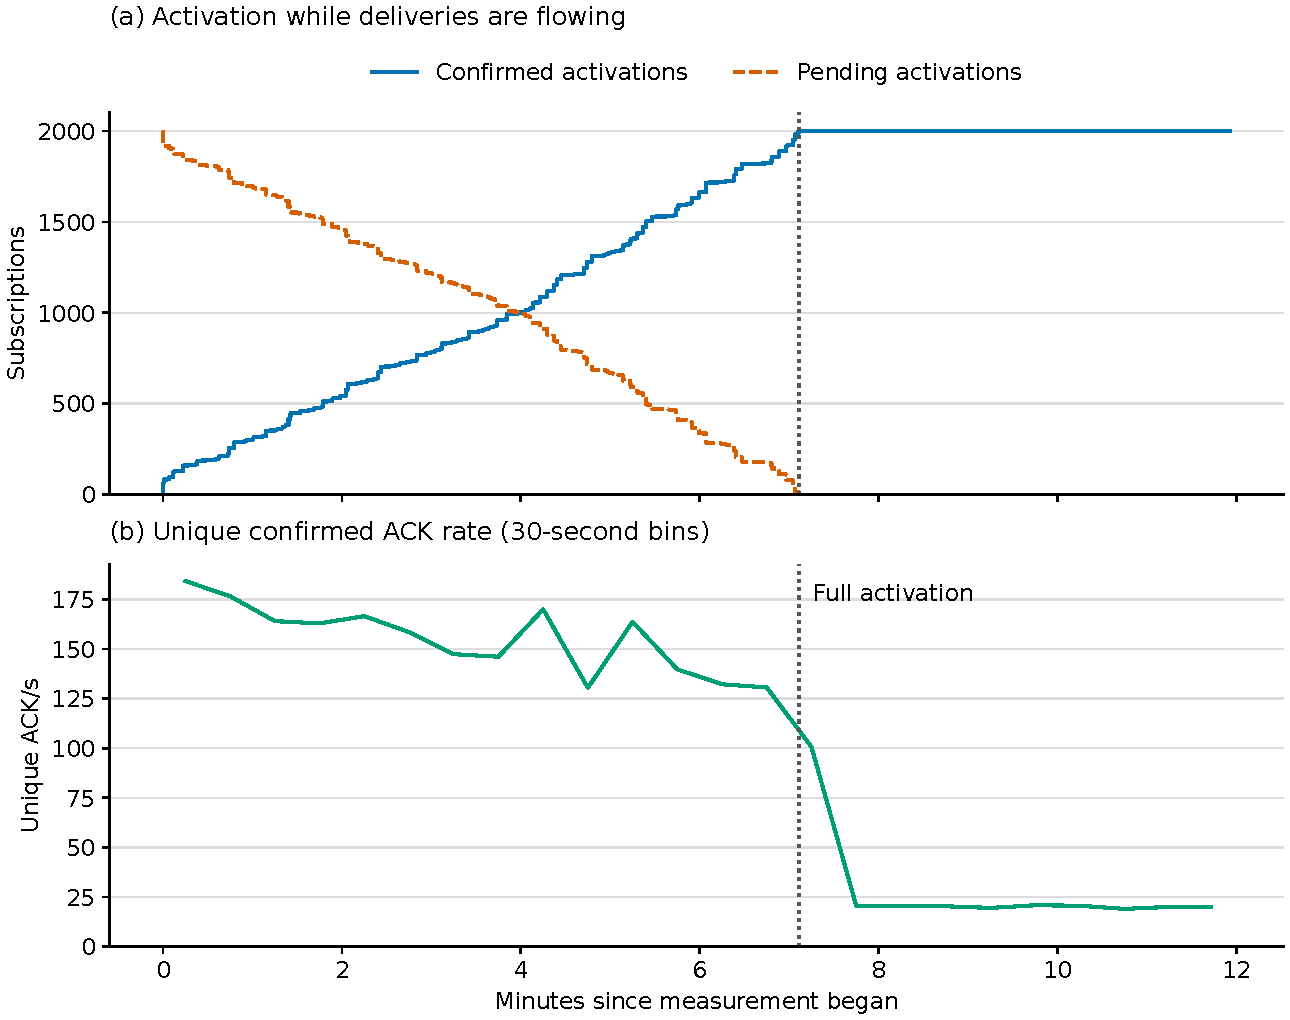
\includegraphics[width=0.94\textwidth]{figures/activation-and-ack-rate.pdf}
  \caption{Activation and acknowledged delivery in the isolated Oracle Cloud cluster run.
  Top: confirmed and pending activation counts. Bottom: distinct observed
  subscription--message pairs whose first successful ACK receipt occurs in
  each 30-second bin, divided by that bin's actual duration. The dotted line
  marks full activation. DQL decisions start after this line.}
  \Description{Activation rises to two thousand while pending activations
  fall to zero. ACKs arrive throughout startup. The later delivery rate falls
  as the consumed workload changes; the curve is not a matched throughput
  comparison with a static policy.}
  \label{fig:mumbai-live-activation}
\end{figure}
\FloatBarrier

Figure~\ref{fig:mumbai-live-activation} retains the startup interval rather
than treating it as discarded warm-up. Of 73,587 distinct first ACKs inside
the 716.017-second measurement window, 66,400 occurred before full activation.
A further 52 attempts completed during shutdown, bringing final reconciled
deliveries to 73,639. The rate curve describes consumption of existing queued
work. It describes startup and workload drainage rather than constant-offered-load
capacity. DQL begins after full activation, so these measurements establish
delivery during startup followed by redistribution. Activation time precedes
the policy intervention.

\begin{figure}[!htbp]
  \centering
  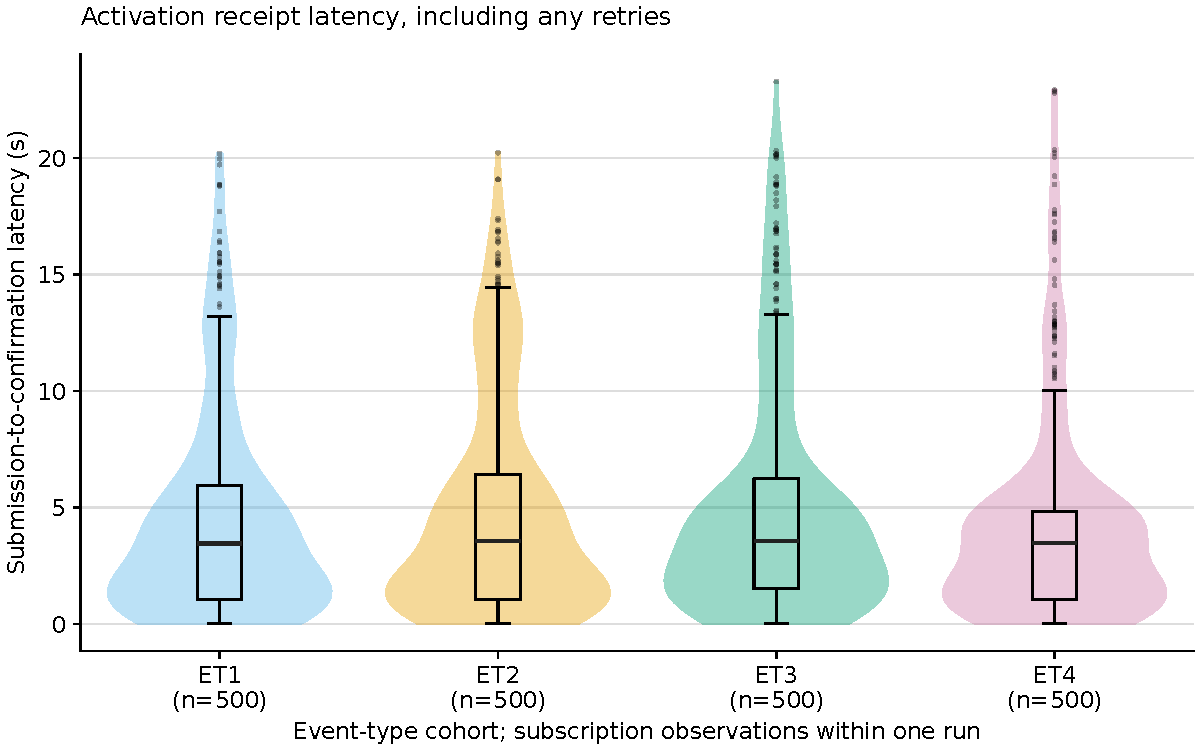
\includegraphics[width=0.92\textwidth]{figures/activation-latency-violin-box.pdf}
  \caption{Within-run activation latency $\ell_k^{\mathrm{act}}=t_k^{\mathrm{ready}}-t_k^{\mathrm{send}}$ for 500 subscriptions
  in each event-type cohort. Violin widths show smoothed empirical density;
  boxes show the interquartile range and median. Whiskers use 1.5 interquartile
  ranges, with observations beyond them retained as points. These are
  subscription observations in one run, not independent cluster trials.}
  \Description{Four violin and box plots show activation receipt latencies.
  Medians are approximately three and a half seconds, with observed upper
  tails reaching roughly twenty to twenty-three seconds.}
  \label{fig:mumbai-activation-latency}
\end{figure}
\FloatBarrier

Figure~\ref{fig:mumbai-activation-latency} distinguishes an individual request's
latency from the time to activate the complete population. Cohort medians were
3.443, 3.560, 3.567 and 3.476 seconds; nearest-rank 99th percentiles were
18.805, 16.907, 20.072 and 20.038 seconds. The subscriptions share upstream services and scheduling conditions, so their
observations are dependent. The distributions describe within-run variation,
without estimating a between-policy confidence interval. A concurrent
thread snapshot found fourteen subscription handlers waiting for upstream
transition confirmation. This locates the observed startup bottleneck in
upstream confirmation waits; the snapshot does not establish CPU saturation.

The complete ledger covers observed delivery attempts, with publisher-to-Queue
event counts outside its scope. This qualification establishes
receipt-confirmed activation under delivery load, probe-based redistribution
with a 60\% reduction in source subscriptions, and reconciled closure. The
recorded delivery rates include workload depletion and startup, so the
experiment reports redistribution rather than an isolated throughput effect.

\subsection{Loaded DQL Migration During Pod Scale-Out}
\label{sec:live-dql-scaleout}

We next tested selective connection replacement during event delivery in a
separate Oracle Cloud cluster run. One client attached 1,000 registered
subscriptions to four persistent connections on one subscriber Pod, with
250 subscriptions per connection. The isolated deployment then grew from
one to four Ready Pods while the same client process remained running.
The second Pod became Ready before standby activation was released; the
third and fourth Pods were added during observation. The transport load
balancer assigned each empty probe to a Pod. The client used the retained
socket only when DQL selected migration and the execution guards passed.

The frozen checkpoint had 9,985 training updates and used $\epsilon=0$.
The trial allowed three executed actions in a configured 600-second window,
with a 60-attempt probe-discovery budget. Telemetry had to satisfy the
180-second age limit and 0.8 minimum backlog coverage. Each Pod requested
1.5 CPU cores and 4~GiB memory, with limits of three cores and 6~GiB.
The client used 32 workers and a fixed one-second processing delay to keep
work outstanding during handoff. This setting tests acknowledgement-aware
migration under a bounded client drain rate, rather than maximum Pod capacity.

Two bounded batches each published four synthetic source events. Each event
matched 5,000 registered subscriptions, including the client's 1,000-subscription
cohort. Thus, publication exposed the queue to 40,000 copies while the measured
cohort accounted for 8,000 delivery attempts. Capacity was checked before each
batch against the existing 400~MB limit, retaining an 80~MB reserve and prior
unreconciled publication costs. No queue purge or quota increase was used.

\begin{table}[!htbp]
  \centering
  \small
  \caption{Executed frozen-DQL handoffs in the loaded Oracle Cloud scale-out
  run. P1 is the initial Pod; P2 and P3 are added Pods. Drain time is included
  in total handoff time. These are three actions within one run.}
  \Description{Three handoffs each move 250 subscriptions and retain the other
  three active sessions. The first two move from P1 to P2; the third moves the
  first group again from P2 to P3. Total times are 97.555, 10.881 and 79.657 seconds.}
  \label{tab:live-dql-loaded-handoffs}
  \begin{tabular}{llrrrr}
    \toprule
    Action & Path & Subscriptions & Other sessions & Drain (s) & Total (s) \\
    \midrule
    H1 & P1 to P2 & 250 & 3 retained & 93.862 & 97.555 \\
    H2 & P1 to P2 & 250 & 3 retained & 8.339 & 10.881 \\
    H3 & P2 to P3 & 250 & 3 retained & 76.166 & 79.657 \\
    \bottomrule
  \end{tabular}
\end{table}

Table~\ref{tab:live-dql-loaded-handoffs} records actual policy execution, not
just a migration recommendation. The three observed differences between the
migration and stay Q-values were 1.7126, 1.2919 and 1.8201. Each migration was
admissible and selected by the frozen network. Before-and-after session maps
show that every handoff preserved the other three active connections. Two
original sessions remained unchanged throughout the run. The mechanism
therefore replaced selected connections without disconnecting the whole pool.

\begin{figure}[!htbp]
  \centering
  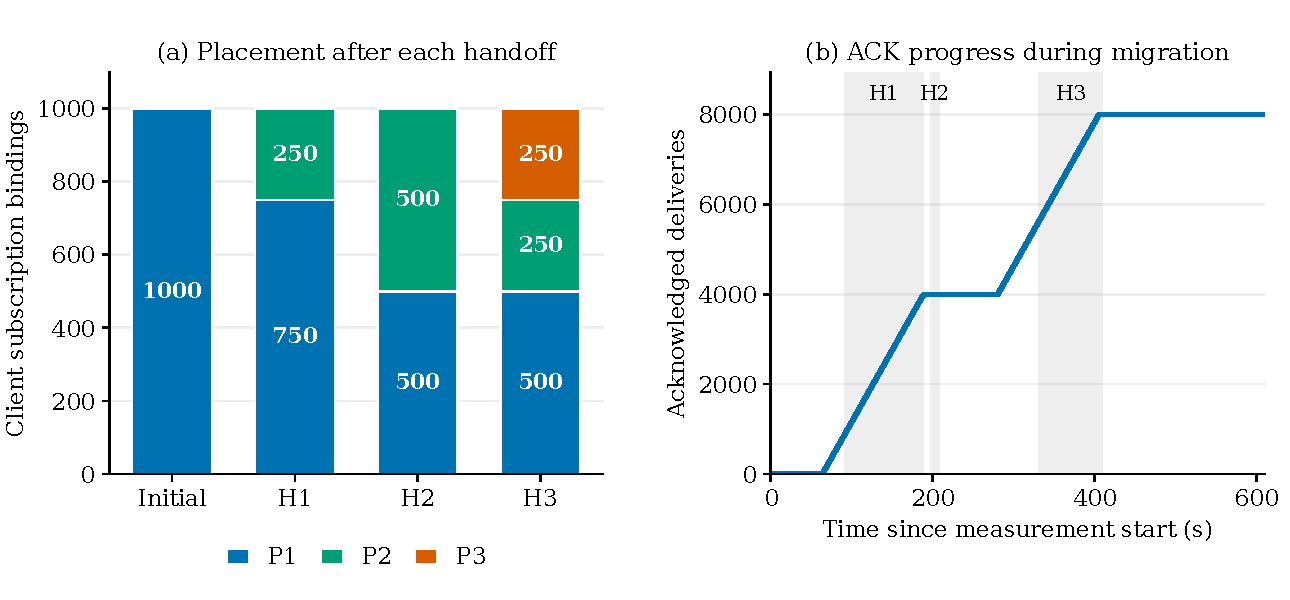
\includegraphics[width=\textwidth]{figures/live-dql-loaded-scaleout.pdf}
  \caption{Measured loaded DQL migration in the Oracle Cloud cluster.
  (a) Receipt-confirmed client bindings at the initial snapshot and after
  H1--H3. Each bar accounts for all 1,000 subscriptions; the four active
  connections each retain 250 subscriptions. P4 has no client bindings and
  is observed only through a probe. (b) Cumulative ACK receipts, aggregated
  in one-second bins. Shaded spans show the measured complete handoff
  intervals, including source drain. The curve describes this bounded
  workload, not a matched between-policy throughput comparison.}
  \Description{Placement changes from one thousand bindings on P1 to seven
  hundred fifty on P1 and two hundred fifty on P2, then five hundred on each,
  and finally five hundred on P1, two hundred fifty on P2 and two hundred fifty
  on P3. ACK receipts reach eight thousand while three shaded handoff intervals
  mark selective connection migration.}
  \label{fig:live-dql-loaded-scaleout}
\end{figure}

Figure~\ref{fig:live-dql-loaded-scaleout}(a) separates moved subscriptions
from handoff operations. H3 moves the group already transferred by H1, so
the three actions comprise 750 subscription-handoff operations involving
500 distinct subscriptions. The final distribution across the four available
Pods is 500, 250, 250 and zero. The maximum client population on one Pod falls
from 1,000 to 500, a 50\% reduction, without increasing the four active
connections. The last Pod remains a probe candidate after the three-action
budget is reached. Discovering it does not automatically promote it.

Figure~\ref{fig:live-dql-loaded-scaleout}(b) uses the confirmed ACK receipt
timestamp of each recorded delivery. Its cumulative total reaches 8,000,
and each of the 1,000 registered subscription hashes has eight acknowledged
delivery records. The ledger contains zero recorded ACK failures, processing
failures, duplicate candidates or unresolved deliveries at clean closure.
Long drain intervals remain visible: source retirement waits for outstanding
work instead of discarding it to shorten the measured handoff. The configured
window contains 60 decision records; its actual measurement boundaries span
609.716 seconds, including boundary handling.

The identity check uses STOMP message identifiers and confirms observed
delivery/ACK accounting. Source CloudEvent identities and individual backend
queue deletions are outside that ledger's scope. A separate unloaded
1,000-subscription run executed two handoffs in 5.244 and 5.172 seconds;
those timings are retained separately because the processing conditions
differ. The online and target weights remained identical to the input
checkpoint in both runs. The loaded run saved 39 valid experience transitions
without applying new training updates. The complete private archive verifies
256 files, and the manuscript figure uses identifier-free aggregates derived
from those records. The isolated deployment was restored to one Ready Pod;
all 13 shared-resource isolation checks passed.

\FloatBarrier

\subsection{TTL-Based Reconnection Under Delivery Load}
\label{sec:ttl-reconnection}

Time-to-live (TTL) reconnection is an existing alternative to client-directed
connection replacement in the subscriber service. It was disabled in the
preceding Oracle Cloud cluster experiments and enabled in the isolated
recovery trials reported below. The deployment
team reported that enabling age-based disconnection under event load caused
widespread delivery interruptions and slow resubscription: delivery restarted
on early-restored subscriptions while the remaining subscriptions were still
being attached. These operational reports provide context rather than a
frequency or severity estimate. The matched-preload trial in
Section~\ref{sec:ttl-preload-results} measures
expiry-related interruptions and ACK completion using server-correlated records.

\subsubsection{Implemented Expiry and Recovery Paths}

The server enables expiry only when the configured connection TTL is positive.
For a connection established at time $t_c^{\mathrm{open}}$, its nominal expiry is
\[
 t_c^{\mathrm{exp}}=t_c^{\mathrm{open}}+T_{\mathrm{TTL}}+60J_c,
 \qquad J_c\in\{1,\ldots,60\},
\]
where $T_{\mathrm{TTL}}$ is in seconds and $J_c$ is the implementation's
uniformly sampled integer jitter in minutes. A scheduled scan runs with a
60-second fixed delay. An expired connection is submitted to a cleanup
executor, its server-side subscription associations are removed, and its
socket is closed. Scheduling and cleanup add delay beyond $t_c^{\mathrm{exp}}$; the scan
interval is not a hard upper bound on closure latency. Several expired
connections can be selected in one scan, although the random jitter reduces
deliberate synchronization. The implementation does not imply that every
client connection expires simultaneously.

The Python client reconnects the affected socket through the transport load
balancer and resends the subscriptions retained for that socket. Recovery applies to the affected connection. It does not automatically
restart the whole client pool. Each
subscription retains its previous delivery state. Consequently, an active
subscription requests active delivery immediately on resubscription; there is
no whole-connection barrier that first restores every subscription and then
releases their events together. Transport reconnection can therefore finish
well before subscription restoration.

This sequence explains the two distinct concerns in the operational report.
First, the expired socket cannot deliver while it is being replaced, and
overlapping recovery intervals can interrupt a large fraction of the pool.
Second, early-restored subscriptions can resume event delivery while other
\texttt{SUBSCRIBE} operations are still outstanding. Delivery and restoration
then overlap in the same service. The server's cleanup also traverses shared
subscription state under a write lock. These operations can compete for shared resources. Their effects on throughput
and latency depend on workload and cannot be inferred from connection age alone.

\begin{table}[!htbp]
  \centering
  \small
  \renewcommand{\arraystretch}{1.18}
  \caption{Implemented TTL reconnection versus guarded DQL migration.
  This compares control mechanisms, not measured performance rankings.}
  \Description{TTL selects connections by age, closes them and reconnects through
  the load balancer. DQL evaluates a retained probe, establishes standby bindings,
  drains the source and activates the replacement before retiring the old socket.}
  \label{tab:ttl-mechanism-comparison}
  \begin{tabular}{p{0.20\linewidth}p{0.34\linewidth}p{0.34\linewidth}}
    \toprule
    Property & Existing TTL strategy & Guarded DQL migration \\
    \midrule
    Trigger & Age, jitter and periodic scan & Observed pressure, Q-values and feasibility guards \\
    Destination & Reconnect assigned by load balancer & Existing load-balancer-assigned probe evaluated before promotion \\
    Replacement & Cleanup and close before reconnect & Target standby before source quiescence and drain \\
    Subscription restart & Retained active subscriptions resume individually & Receipt-gated handoff and controlled target activation \\
    In-flight work & No DQL drain barrier in TTL closure path & Source drain checked before retirement \\
    Scope & Every connection eligible by expiry time & Bounded selected connection; other sockets retained \\
    \bottomrule
  \end{tabular}
\end{table}
\FloatBarrier

Table~\ref{tab:ttl-mechanism-comparison} identifies the intended advantage of
probe-guided migration: destination evaluation and subscription handoff happen
before the old socket is retired. TTL can also reach a newly added Pod, but
selects by connection age rather than the destination's subscription or backlog
pressure. DQL evaluates that pressure and controls source retirement; its
handoff duration still includes source drain and target activation, so delivery
can pause during the transfer.

\subsubsection{Recovery Endpoints and Verification}

Let $d_c$ be the observed disconnect time, $h_c$ the replacement
\texttt{CONNECTED} time, and $r_c$ the time when all retained subscriptions
have successful replacement-session receipts. The two recovery endpoints are
\[
 T_c^{\mathrm{conn}}=h_c-d_c, \qquad T_c^{\mathrm{restore}}=r_c-d_c.
\]
If recovery is incomplete at the next disconnect or the end of observation,
we record only the elapsed waiting time. This is a right-censored observation,
not a successful fast reconnect. Let $s$ denote elapsed trial time in seconds,
and let $I_c(s)$
equal one while connection $c$ is disconnected or its retained bindings remain
unrestored, and zero otherwise. With $\mathcal{C}_0$ denoting the active
connection pool at the start of a TTL trial, the affected fraction is
\[
 F(s)=\frac{1}{|\mathcal{C}_0|}
 \sum_{c\in\mathcal{C}_0} I_c(s).
\]
The peak of $F$ and its time integral distinguish a brief single-socket outage
from widespread or prolonged recovery. Delivery-rate degradation on sockets
that remain connected is measured separately; it is not counted as a physical
disconnect. We also measure unique receipt-confirmed ACK rate, gaps between deliveries,
pending subscription count, and receipt latency per subscription. These show
the effects on both event delivery and subscription operations. Events delivered before $r_c$
directly establish overlap between delivery and incomplete restoration, but
overlap alone does not prove CPU or network saturation.

The recovery instrumentation requests receipts for reconnect subscriptions
without serializing their dispatch. It preserves pending caller Futures,
distinguishes successive sessions, and stores timestamps alongside the exact
delivery ledger. A common instrumentation contract defines the measurements
across comparison arms.
Client disconnects are attributed to TTL only when matched to server expiry
records; unrelated network failures remain separate.

The implementation-level checks exercise the disabled TTL branch, expired
connection closure, and selection of expired rather than unexpired sockets
in a common scan. Client checks cover receipt ownership, unchanged delivery
states, interrupted recovery, and censored timing analysis. These checks
validate implementation behavior. The live comparisons reported below measure
expiry-related interruptions, receipt completion, and recovery timing using
the native jitter. This separates observed behavior from an artificial
simultaneous-disconnection scenario.

\subsubsection{Recovery Observed Within the Existing Storage Limit}

The isolated recovery trial retained the installed 400,000,000-byte Queue
limit and consumed existing experimental events without a storage increase
or new publication. Four clients attached 1,250 subscriptions each to one
subscriber Pod, giving 5,000 receipt-confirmed standby subscriptions across
20 delivery connections and four probes. Each delivery connection held 250
subscriptions. Activation then released delivery with a bounded window of
16 outstanding requests per client. Native TTL used a configured value of
60 seconds with the original 1--60-minute jitter and scheduled scan; no
simultaneous-disconnection rule was introduced.

A sealed client record captures a complete recovery of 250 retained
subscriptions. The replacement socket reached \texttt{CONNECTED} in
0.018 seconds, whereas receipt-confirmed restoration took 104.174 seconds.
During that restoration interval, 82 delivery attempts arrived on the
replacement session. Thus, transport recovery did not mean that the
subscription population was ready, and delivery demonstrably overlapped
with restoration. The corresponding server expiry record was not retained. We therefore report
this as recovery during a TTL-enabled trial, not as a disconnect independently
confirmed to have been caused by TTL. A second client record does match an
explicit server TTL-close request by session identity and records the
subsequent disconnect; this partial run confirms that native expiry occurred, but it is not a
completed performance trial.

The TTL-enabled execution ended during activation after a receipt timeout.
One client sealed its evidence; the supervisor's earlier cleanup deadline
interrupted the other three before sealing. These records are retained as
diagnostics rather than treated as four successful repetitions. ACK errors
also occurred on connections without a recorded disconnect, so they are not
all assigned to TTL. The observed recovery sequence supports distinguishing
socket readiness, subscription readiness and delivery activity; it does not
by itself estimate a TTL-versus-DQL throughput effect.

After restoring TTL to its disabled state, a functional control used the same
5,000-subscription population and existing events. Its four verified client
records contain 117,269 delivery attempts, 110,411 receipt-confirmed ACKs and
6,858 unresolved attempts. No active-connection interruption was recorded,
but activation ended after an explicit upstream state-transition failure
exhausted its retry budget; 2,929 bindings had confirmed active state in the
last progress records. This distinguishes the expiry/recovery mechanism from
an activation bottleneck that also occurs without TTL. Because the first
execution had already consumed part of the workload, the two runs do not
provide a matched-backlog throughput comparison. Both preserve the frozen
model without additional training. The isolated Deployment was restored,
and all thirteen shared-resource isolation checks passed.

% Live measurements only. Derived figures and aggregates retain the sealed
% September 25 evidence hashes; simulator results are not pooled with this pair.
\subsubsection{Native TTL During Two Delivery Bursts}
\label{sec:ttl-loaded-results}

Before the preload trial, a separate live pair tested native TTL against a
static TTL-disabled control on one isolated Oracle Cloud subscriber Pod.
Both arms used 5,000 subscriptions, five clients, 20 occupied connections and
five empty probes, with zero artificial client processing delay. Each started
from an empty Queue and received two bursts of three accepted source events,
giving 30,000 recorded delivery attempts per arm. Both used the same server
image and 900-second post-activation observation. Native TTL retained its
original jitter. The control replayed the accepted burst schedule: its first
requests were 0.462 and 0.578 seconds later than the native relative targets
of 26.182 and 319.207 seconds. Queue-statistics budget failures stopped other
publication blocks before any event attempt; those failures were retained.

\begin{table}[!htbp]
 \centering
 \small
 \renewcommand{\arraystretch}{1.14}
 \caption{Oracle Cloud two-burst TTL comparison, separate from the subsequent
 preload pair. Both arms use static placement on one Pod; TTL off is not a
 learned DQL intervention. Latency statistics include confirmed ACKs only.}
 \Description{Native TTL records five interruptions, 369 unresolved receipts
 and a 238.392-second confirmed ACK latency p95. The static TTL-disabled control
 records zero interruptions, no unresolved receipts and a 55.826-second p95.}
 \label{tab:ttl-loaded-results}
 \begin{tabular}{p{0.51\linewidth}rr}
  \toprule
  Measurement & Native TTL & Static TTL off \\
  \midrule
  Delivery attempts & 30,000 & 30,000 \\
  Receipt-confirmed ACKs & 29,631 & 30,000 \\
  Unresolved ACK receipts & 369 & 0 \\
  Server-matched TTL interruptions & 5 & 0 \\
  Confirmed ACK latency: median (s) & 19.439 & 21.407 \\
  Confirmed ACK latency: 95th percentile (s) & 238.392 & 55.826 \\
  Clients with receipt-complete shutdown & 2 of 5 & 5 of 5 \\
  \bottomrule
 \end{tabular}
\end{table}

Table~\ref{tab:ttl-loaded-results} shows the tail that a median alone would
miss: native TTL's confirmed-ACK p95 was 4.27 times the control's, although its
median was 1.968 seconds lower. Five interruptions matched server expiry records.
Transport reconnection took 17--24~ms, whereas restoring all 250 bindings on
each affected connection took 0.504--0.973 seconds. One recovery received
22 delivery callbacks before all binding receipts arrived. This directly
demonstrates delivery overlapping resubscription within the observed short
recovery windows; prolonged stalls and whole-pool expiry were not observed. All 369 unresolved
attempts belonged to expired sessions; three clients reached the 120-second
receipt-drain deadline. Missing receipts are not counted as lost Queue events.
All ten sealed client bundles were recovered and verified. This single
sequential pair measures TTL-related disruption and confirmed-receipt latency
under static placement. It estimates neither repeated-run capacity nor a
DQL-specific effect.

\subsubsection{Matched-Preload Comparison in the Oracle Cloud Cluster}
\label{sec:ttl-preload-results}

A subsequent isolated trial compared native TTL with the frozen DQL controller
under the same initial queued workload. Each arm used the same 5,000 registered
ET1 subscriptions: five clients held 1,000 subscriptions each on four occupied
connections, with 250 subscriptions per connection and one empty probe per
client. All 20 occupied connections initially terminated on one subscriber Pod.
Three identical Pods became Ready before activation. Each Pod had a limit of
three CPU cores and 6~GiB memory, and both arms used the same pinned server image.
The installed Queue limit remained 400,000,000 bytes; shared subscriber
resources were not changed.

All bindings were attached in standby before six source events were published
through the authenticated ingest path. A pre-activation Queue snapshot verified
30,000 visible copies and zero in-flight copies in each arm. The recorded
delivery ledger subsequently contained six attempts for every subscription in
the same 5,000-subscription cohort. Native TTL retained the 60-second base,
1--60-minute random jitter and scheduled scan. The DQL arm disabled TTL and
loaded unchanged online and target networks from the checkpoint with 9,985
training updates; exploration and further learning were disabled. Observation
continued for 900 seconds after activation, with activation itself also recorded.

The original workload included a six-event refill at five minutes. Its first
Queue-statistics budget check returned HTTP~429 before any event was attempted.
Before the DQL arm started, the comparison was amended to use the six-event
preload without refill. Three DQL preload budget checks also failed before
publication; cooldown and fresh checks admitted the remaining events while all
bindings stayed in standby. The initial copy counts therefore matched, but the setup proceeded at
different rates. Queue occupancy was approximately 20.3~MB in both arms, not
400~MB. This sequential pair measures fixed-preload drainage. Sustained
arrivals and subscriber saturation are outside that workload.

\subsubsection{Receipt Completion and Connection Recovery}

Table~\ref{tab:ttl-preload-results} reports the observed outcomes. Let
$D_{\mathrm{obs}}$ be the number of recorded delivery attempts and
$A_{\mathrm{conf}}$ the number with a confirmed ACK receipt. Receipt completion is
$A_{\mathrm{conf}}/D_{\mathrm{obs}}$; the remainder is unresolved, not classified as
event loss. Both arms recorded 30,000 attempts. Native TTL confirmed 26,831 ACKs
(89.44\%), compared with 30,000 (100\%) in the TTL-disabled arm, a difference of
10.56 percentage points in this pair. The latter arm is labelled
\emph{guard-held DQL}: its controller ran, but telemetry guards held every
decision at \emph{stay}, as explained below.

\begin{table}[!htbp]
 \centering
 \small
 \renewcommand{\arraystretch}{1.14}
 \caption{Measured Oracle Cloud outcomes for the matched 5,000-subscription
 preload. The DQL arm had TTL disabled and executed no migration. Latencies
 are conditional on confirmed ACKs; unresolved receipts are reported separately.}
 \Description{Both arms record thirty thousand delivery attempts. Native TTL
 has twelve server-matched interruptions and 3,169 unresolved receipts. The
 guard-held DQL arm has neither, but executes no migrations.}
 \label{tab:ttl-preload-results}
 \begin{tabular}{p{0.49\linewidth}rr}
  \toprule
  Measurement & Native TTL & Guard-held DQL \\
  \midrule
  Delivery attempts & 30,000 & 30,000 \\
  Receipt-confirmed ACKs & 26,831 & 30,000 \\
  Unresolved ACK receipts & 3,169 & 0 \\
  Receipt completion (\%) & 89.44 & 100.00 \\
  Server-matched TTL interruptions & 12 & 0 \\
  Distinct occupied sockets interrupted & 11 of 20 & 0 of 20 \\
  Peak simultaneously recovering sockets & 3 of 20 & 0 of 20 \\
  Incomplete-restoration exposure (connection-s) & 10.983 & 0 \\
  Confirmed ACK latency: median (s) & 69.862 & 69.836 \\
  Confirmed ACK latency: 95th percentile (s) & 251.546 & 249.874 \\
  Executed DQL migrations & Not applicable & 0 \\
  \bottomrule
 \end{tabular}
\end{table}

All twelve native interruptions matched server expiry records by session
identity and disconnect time. They affected eleven distinct occupied sockets,
with at most four interrupted within a rolling minute. At most three sockets
were concurrently unrestored, giving $\max_s F(s)=3/20=0.15$ and
$\int\sum_c I_c(s)\,ds=10.983$ connection-seconds. Complete binding
restoration took 0.492--1.835 seconds. These observations show overlapping
recovery periods affecting part of the pool, rather than a whole-pool outage. All 3,169 unresolved native
attempts belonged to sessions with matched expiries, but a missing ACK receipt
does not reveal whether the underlying Queue deletion succeeded.

\begin{figure}[!htbp]
 \centering
 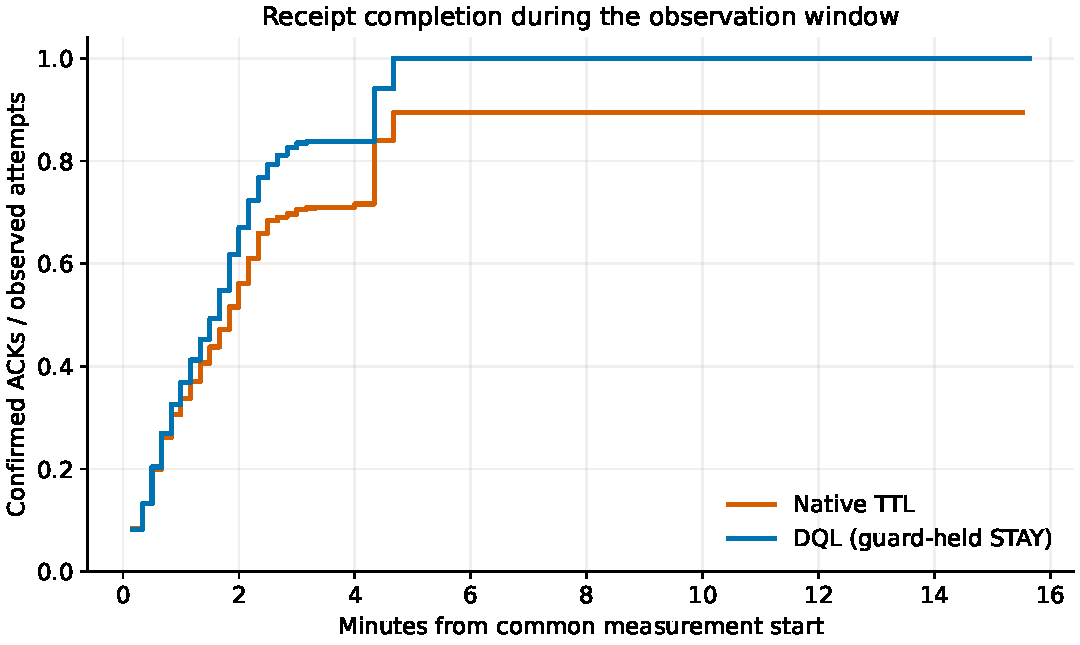
\includegraphics[width=0.88\textwidth]{figures/ttl-preload-ack-completion.pdf}
 \caption{Receipt completion in the Oracle Cloud matched-preload pair.
 Each curve accumulates confirmed ACKs in ten-second bins and divides by all
 30,000 observed attempts in its arm. Unresolved attempts remain in the
 denominator. DQL denotes the guard-held, TTL-disabled execution, not a
 completed migration comparison.}
 \Description{Native TTL receipt completion reaches 89.44 percent and the
 guard-held DQL arm reaches 100 percent. The horizontal axis is minutes from
 the common measurement start within each arm.}
 \label{fig:ttl-preload-completion}
\end{figure}

Figure~\ref{fig:ttl-preload-completion} retains the unresolved attempts in the
final level rather than rescaling each curve using only successful attempts.
Time starts when all five client observation windows overlap within each arm. Those common windows lasted 931.347 and 937.743 seconds,
respectively. Their mean confirmed-ACK rates were 28.809 and 31.992/s, including
idle time; these are whole-window completion rates, not estimates of maximum
Pod bandwidth. Four native clients reached the 120-second final ACK-drain
deadline. We retain their incomplete drains and the coordinator's nonzero exit status
as outcomes. All ten client evidence bundles were sealed and verified;
the DQL coordinator completed cleanly.

\begin{figure}[!htbp]
 \centering
 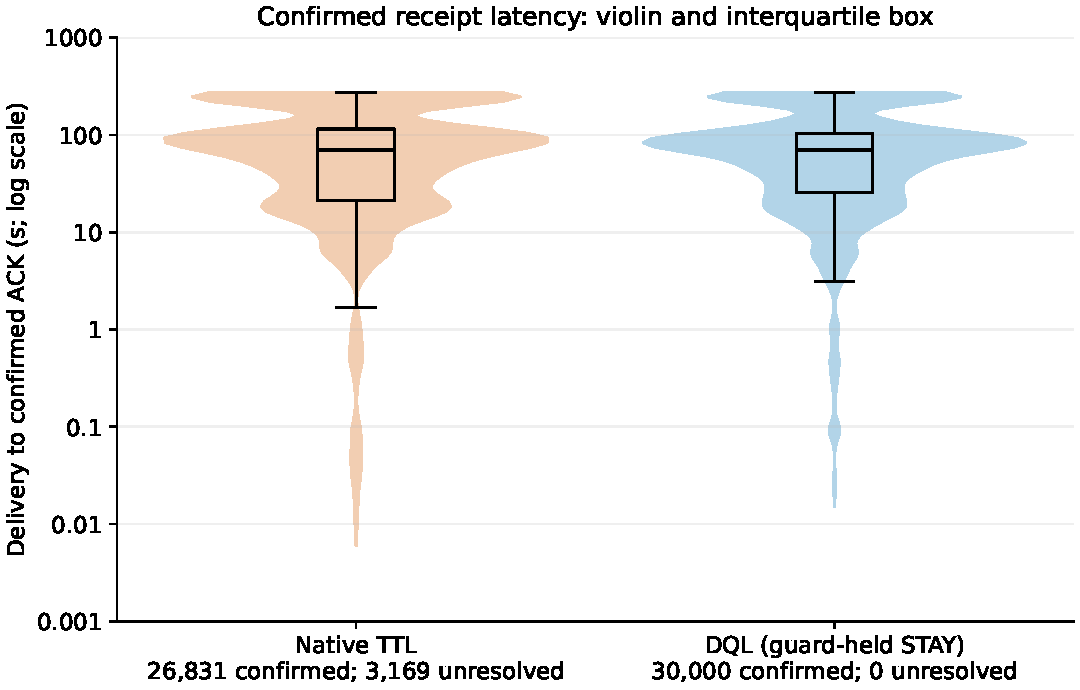
\includegraphics[width=0.88\textwidth]{figures/ttl-preload-ack-latency-violin-box.pdf}
 \caption{Confirmed delivery-to-ACK latency in the Oracle Cloud preload pair.
 Violin density is estimated on $\log_{10}$ latency; boxes show its median and
 interquartile range, with 1.5-IQR whiskers. Outlier markers are suppressed,
 not removed from the observations. Counts exclude unresolved receipts.}
 \Description{Violin and box plots compare 26,831 confirmed native TTL
 latencies with 30,000 guard-held DQL latencies. Their medians are approximately
 seventy seconds. Native TTL additionally has 3,169 unresolved receipts.}
 \label{fig:ttl-preload-latency}
\end{figure}

Figure~\ref{fig:ttl-preload-latency} separates receipt completion from
conditional latency. The confirmed medians differ
by only 0.026 seconds, and the 95th percentiles are also close. Native unresolved
receipts are absent from this latency distribution but remain explicit in
Table~\ref{tab:ttl-preload-results}. Violin width describes within-run latency
variation. The five clients and 30,000 attempts belong to one pair rather than
independent trials, so between-run uncertainty is not estimated. Unlike the
earlier 104.174-second diagnostic, this pair recorded no new delivery callbacks
during subscription-restoration windows. It captures a different recovery
condition from resubscription under concurrent delivery.

\subsubsection{Telemetry Freshness and Action Eligibility}

The DQL trace contains 450 decision intervals, all held at \emph{stay} by
\texttt{invalid-backlog-telemetry}. No migration executed, and all 5,000 bindings
remained on the source Pod despite four Pods being Ready. Statistics collection
paced individual subscription requests at 40~ms for a 5,000-subscription sweep.
Even before network delay or retries, the sweep required at least
$5{,}000\times0.040=200$ seconds, exceeding the 180-second oldest-sample deadline.
The minimum coverage across the Pod and occupied-connection components ranged
from 0.560 to 0.808. Only ten observations met every 80\% coverage threshold;
their oldest constituent samples were 183.127--185.974 seconds old and failed
freshness. A recently received telemetry frame can therefore contain stale
Queue observations. Queue-statistics rate limits further constrained coverage.

This finding separates two operational properties. Native expiry produced
measurable interruptions and receipt uncertainty; the TTL-disabled, guard-held
arm preserved its occupied sockets and completed all observed ACKs. Freshness
checks held migration inactive, so the measured benefit concerns connection
retention and receipt completion, rather than throughput from added Pod
capacity. The checkpoint and guards stayed fixed throughout the trial.
Cleanup verified empty Queue and
dead-letter Queue inventories, restored isolated TTL to zero and one Ready Pod,
and passed all thirteen shared-resource isolation checks.
\FloatBarrier


